
\subsection{Entstehung einer elektromagnetischen Welle}\label{cha:2_sub_Entstehung_einer_Welle}

Die Entstehung einer elektromagnetischen Welle, ausgehend von einem Dipol beispielsweise, beruht auf der Wechselwirkung elektrischer und magnetischer Felder. Vereinfacht beschrieben führt ein Leitungsstrom zwischen einem Paar entgegengesetzter Ladungen (Dipol), zur Induktion eines Magnetfeldes, welches seinerseits wieder ein elektrisches Feld hervorruft. Im Verlauf des Ladungsausgleiches nimmt der Leitungsstrom und damit ebenfalls das Magnetfeld immer weiter ab. Diese zeitliche Änderung des magnetischen Feldes induziert gemäß des Induktionsgesetzes jedoch wiederrum ein elektrisches Feld entgegengesetzter Polarität, welches die beiden betrachteten Körper erneut auflädt. Der Leitungsstrom zwischen den Körpern fließt als Verschiebungsstrom\footnote{Verschiebungsströme beruhen im Gegensatz zu Leitungsströmen nicht auf dem Fluss von Ladungsträgern, sondern auf der zeitlichen Änderung elektrischer Felder und sind somit auch zwischen Raumpunkten ohne direkte Verbindung durch einen Leiter möglich. Der Begriff wurde durch J.C. Maxwell als Ergänzung zum Durchflutungsgesetz nach A.M. Ampére bekannt~\cite{Feldtheorie_Begriffe}} wieder zurück, sodass ein geschlossener Stromkreis entsteht. Dieser periodische Schwingkreis führt zu einer Ausbreitung gekoppelter elektrischer und magnetischer Felder im Raum, was als elektromagnetische Welle bekannt ist. Für die Ausbreitung ist dabei kein umgebendes Medium notwendig~\cite{EM_Schirmung}.
\par
\vspace{\linespace}
Wie in einem Schwingkreis aus Kapazität und Induktivität schwingt die im System vorhandene Energie zwischen den beiden unterschiedlichen Feldern hin und her. Im Verlauf der weiteren Betrachtungen wird, insofern nicht anders erwähnt, von einer harmonischen Schwingung ausgegangen.
\par
\vspace{\linespace}
Bei den sich im Raum ausbreitenden Feldern handelt es sich um reine Wirbelfelder mit in sich geschlossenen Feldlinien \cite{Feldtheorie_Begriffe} (vgl.~\Abb\ref{fig:2_Hertzscher_Dipol}). Für Magnetfelder ist dies ohnehin stets der Fall und da die elektrischen Felder aufgrund zeitlich veränderlicher magnetischer Flüsse entstehen, treten diese ebenfalls in Form von Wirbelfeldern auf~\cite{EM_Schirmung, Feldtheorie_Begriffe}. In der Nähe eines Dipols, also der Ursache der Welle, überlagern sich die Wirbelfelder mit dem elektrischen Quellenfeld, das aufgrund des Ladungsunterschieds auftritt~\cite{EM_Schirmung}. 
\par
\vspace{\linespace}
Wird für die Betrachtung ein infinitesimal kleiner Dipol verwendet, wird dieser Hertz'scher Dipol genannt und stellt die einfachste Form einer Antenne dar. Zur theoretischen Betrachtung kann jede weitere, beliebige Antennenform aus Hertz'schen Dipolen superponiert werden \cite{EM_Schirmung}.

\begin{figure}[ht]
    \centering
    \begin{subfigure}[b]{0.4\textwidth}
        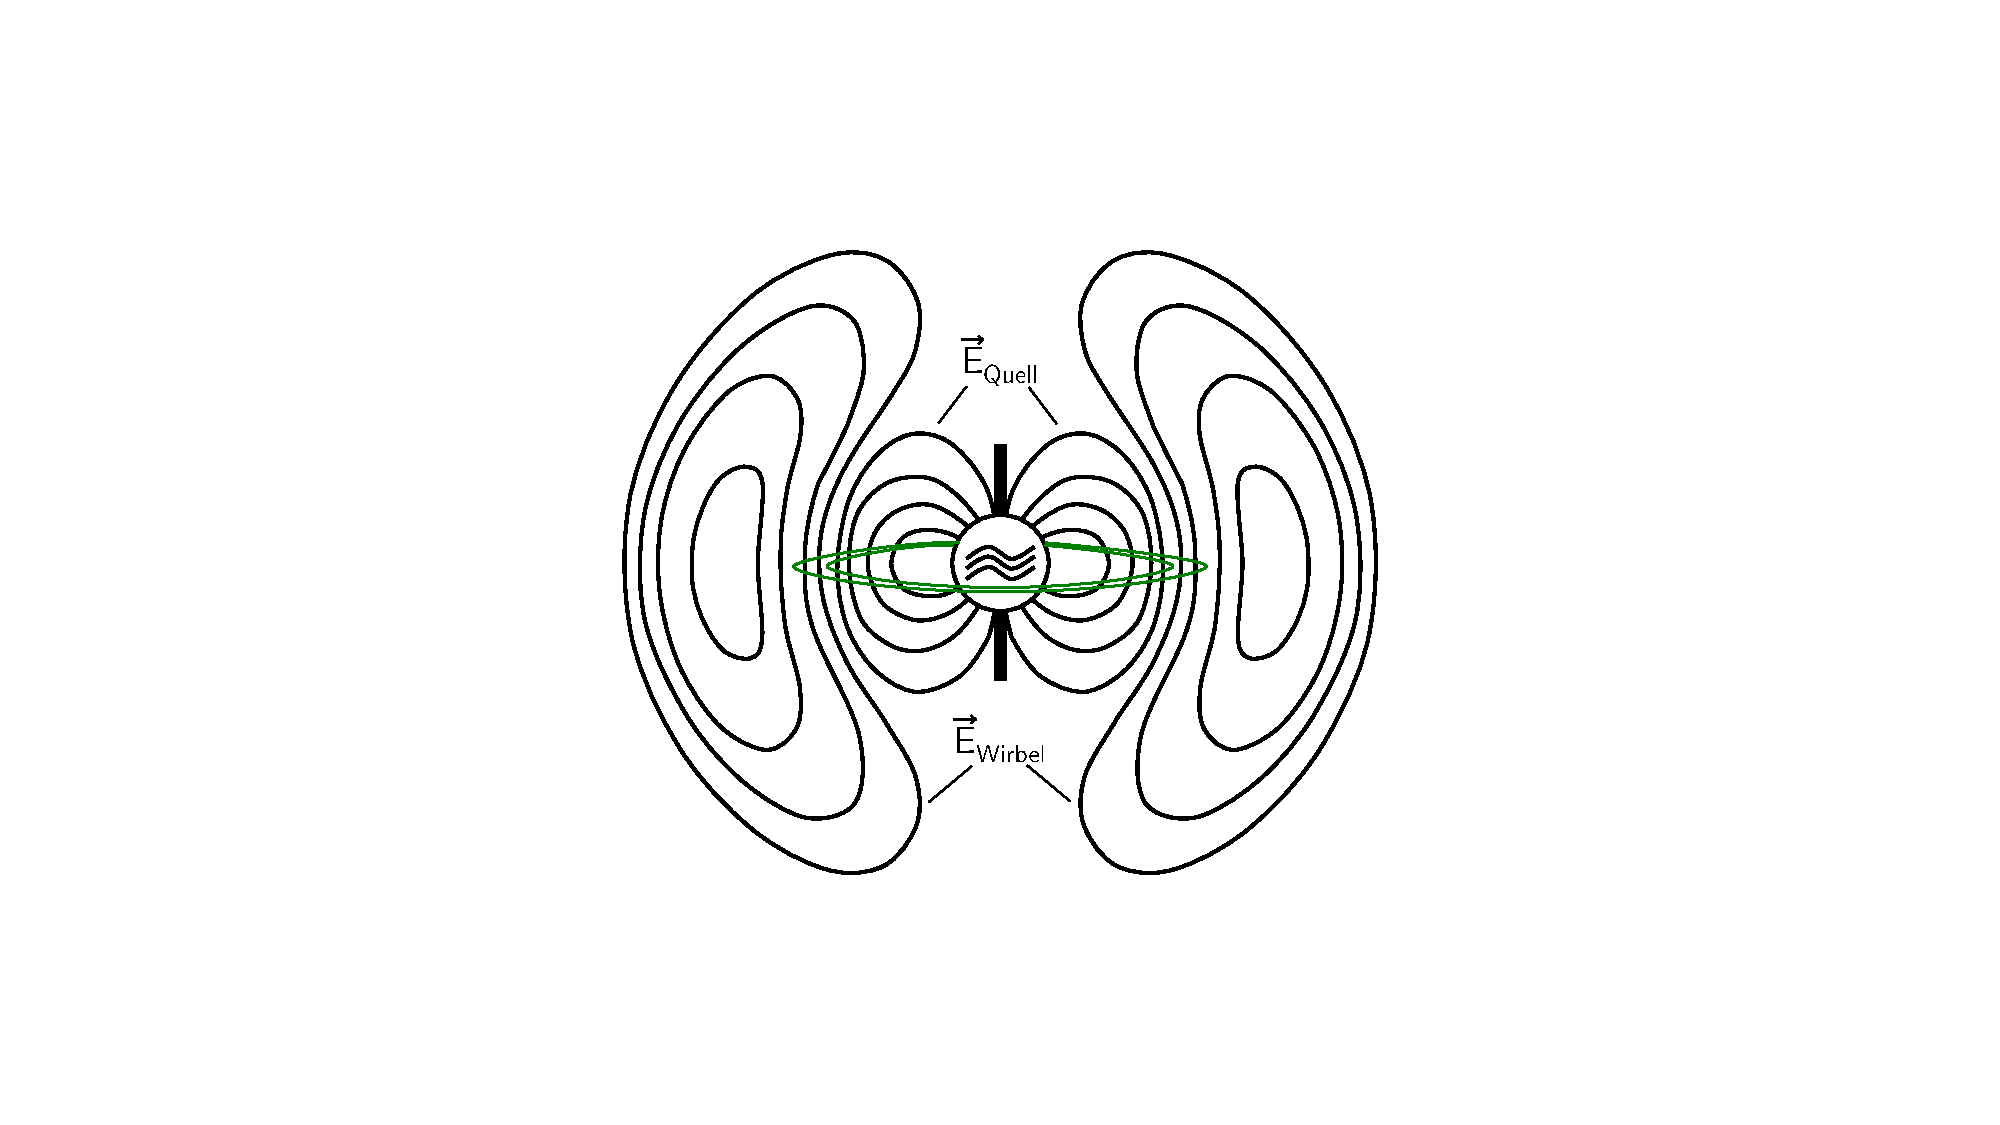
\includegraphics[page = 1, height=0.2\textheight, trim = 10cm 4cm 9.5cm 4cm, clip]{Abbildungen/Kapitel2/Hertz-Dipol.pdf}
        \caption{Wirbelfeldlinien in Momentaufnahme}\label{subfig:2_Hertzscher_Dipol_A}
    \end{subfigure}
    \hspace{1cm}
    \begin{subfigure}[b]{0.4\textwidth}
        \includegraphics[page = 2, height=0.2\textheight, trim = 4.5cm 0cm 8cm 0cm, clip]{Abbildungen/Kapitel2/Hertz-Dipol.pdf}
        \caption{Ebene Welle}\label{subfig:2_Hertzscher_Dipol_B}
    \end{subfigure}
    \caption[Schematische Darstellung eines Hertz'schen Dipols]{Schematische Darstellung eines Hertz'schen Dipols nach~\cite{EM_Schirmung}. Die dargestellte ebene Welle (b) bildet sich in ausreichend großer Entfernung von der Quelle aus}
    \label{fig:2_Hertzscher_Dipol}
\end{figure}


\subsection{Feldverlauf in der Umgebung eines Dipols}\label{cha:2_sub_Feldverlauf_in_Umgebung_eines_Dipols}

Um die Charakteristik des umgebenden Feldes eines Dipols zu bestimmen ist es zielführend, die Komponenten der Feldstärken in Abhängigkeit des Abstandes zu betrachten. Da die Strahlungsfelder jeder Antenne endlicher Abmessung sphärische Wellen sind \cite{Antenna_Theory}, ist eine Betrachtung in Kugelkoordinaten $\left(r, \phi, \theta\right)$ zweckmäßig (vgl.~\Abb \ref{fig:2_Feldverlauf}). 

\begin{figure}
    \centering
    \begin{subfigure}[b]{0.4\textwidth}
        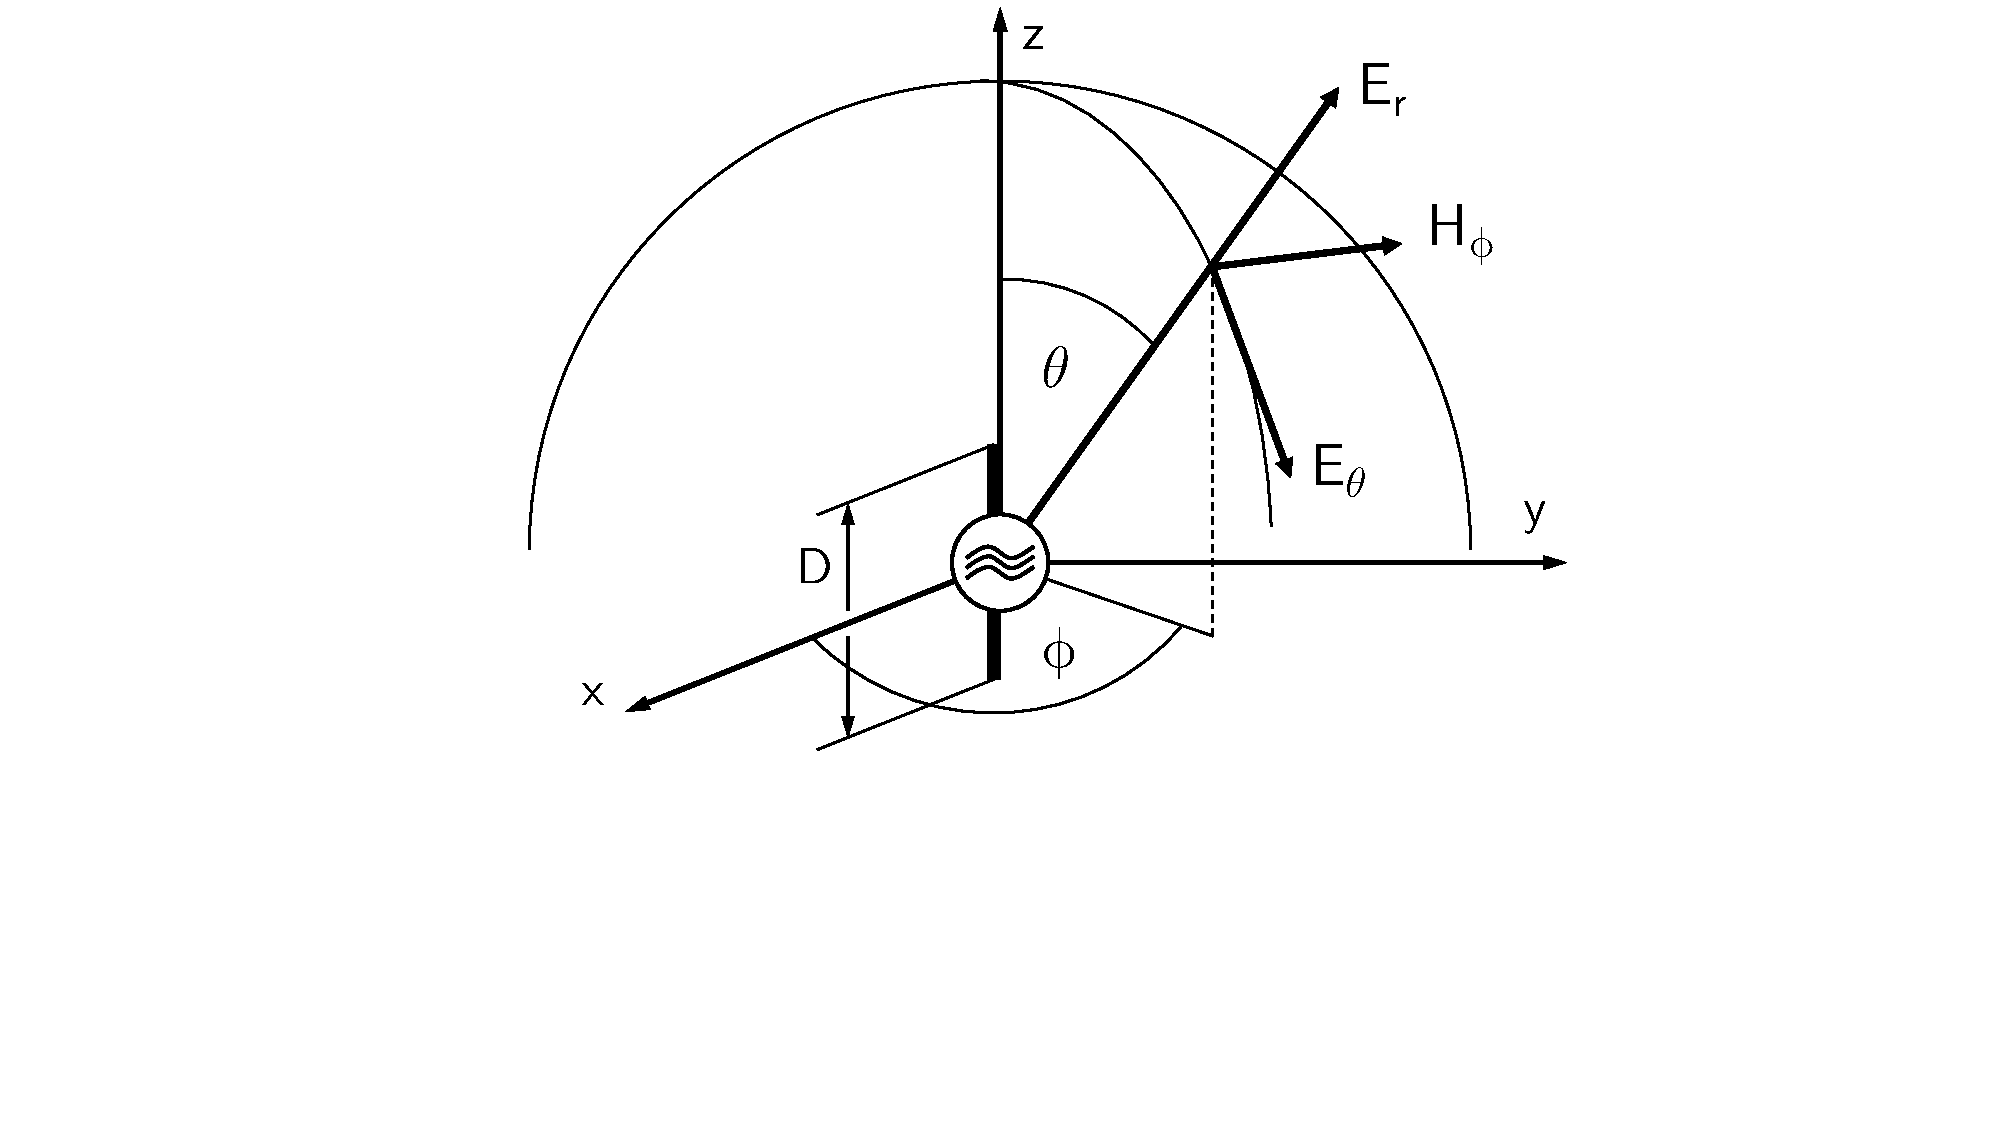
\includegraphics[page = 1, height=0.2\textheight, trim = 8.5cm 5cm 7cm 0cm, clip]{Abbildungen/Kapitel2/Hertz'scher_Dipol.pdf}
        \caption{\label{subfig:2_Feldverlauf_Koordinatensystem}}
    \end{subfigure}
    \hspace{1cm}
    \begin{subfigure}[b]{0.4\textwidth}
        \includegraphics[page = 2, height=0.2\textheight, trim = 8.5cm 3cm 7cm 2cm, clip]{Abbildungen/Kapitel2/Hertz'scher_Dipol.pdf}
        \caption{\label{subfig:2_Feldverlauf_Hertz-Dipol}}
    \end{subfigure}
    %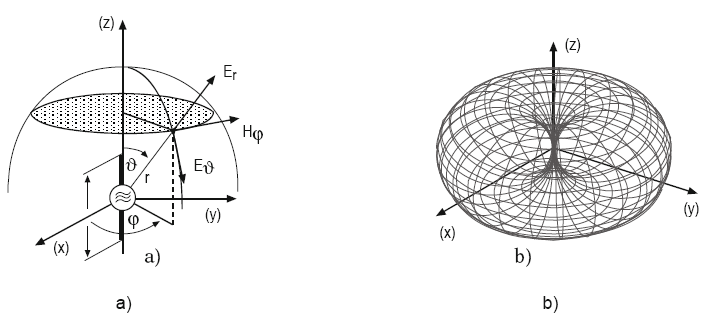
\includegraphics[width=.8\textwidth]{Abbildungen/Kapitel2/Feldverlauf.png}
    \caption[Schematische Darstellung eines Dipols und Nahfeldumgebung eines Hertz'schen Dipols]{Schematische Darstellung eines Dipols mit Feldvektoren im Kugelkoordinatensystem und Feldlinienverlauf in Nahfeldumgebung eines Hertz'schen Dipols nach~\cite{EMV}}
    \label{fig:2_Feldverlauf}
\end{figure}

Für die Amplituden der Feldvektoren, die im Allgemeinen komplex sind, lassen sich demnach folgende Ausdrücke bestimmen~\cite{Antenna_Theory, EMV}:

\begin{subequations}
\label{eq:2_elektrische_Feldvektoren}
    \begin{align}
        E_r &= \frac{\hat i D \sqrt{\frac{\mu_0}{\varepsilon_0}} \lambda \cos{\theta}}{j 4 \pi^2 r^3}\left(1+ j\frac{2\pi}{\lambda}r\right)e^{-j\frac{2\pi}{\lambda}r} \label{subeq:2_E-Feld1} \\
        E_{\phi} &= 0 \label{subeq:2_E-Feld2} \\
        E_{\theta} &= \frac{\hat i D \sqrt{\frac{\mu_0}{\varepsilon_0}} \lambda \sin{\theta}}{j 8 \pi^2 r^3}\left(1+ j\frac{2\pi}{\lambda}r + \left(j\frac{2\pi}{\lambda}r\right)^2\right)e^{-j\frac{2\pi}{\lambda}r} \label{subeq:2_E-Feld3}
    \end{align}
\end{subequations}

\begin{subequations}
\label{eq:2_magnetische_Feldvektoren}
    \begin{align}
        H_r &= 0 \hphantom{\text{DiesIstEinLangesPlatzhalterwort1111111111}} \label{subeq:2_H-Feld1}\\
        H_{\phi} &= \frac{\hat i D \sin{\theta}}{4 \pi r^2}\left(1+j\frac{2\pi}{\lambda}r\right)e^{-j\frac{2\pi}{\lambda}r} \label{subeq:2_H-Feld2}\\
        H_{\theta} &= 0
    \end{align}
\end{subequations}

Die \Gleichungen\eqref{eq:2_elektrische_Feldvektoren} und~\eqref{eq:2_magnetische_Feldvektoren} sind im gesamten Gebiet bis auf die Quelle selbst gültig \cite{Antenna_Theory}. Mit ihnen lassen sich Interpretationen bezüglich der Eigenschaften einer Antennenumgebung vornehmen:
\par
\vspace{\linespace}
Bei Abständen $r< \lambda / 2\pi$ beginnen die Terme höherer Ordnung zu dominieren. Diese Umgebung wird als Nahfeld bezeichnet und bei der dort befindlichen Energie handelt es sich hauptsächlich um imaginäre, d.h. gespeicherte Energie \cite{Antenna_Theory}. Das Nahfeld kann nach~\cite{Bundesnetzagentur_Glossar_Nahfeld} weiterhin in reaktives und strahlendes Nahfeld, auch als Übergangsfeld bezeichnet, unterteilt werden. Für Antennen beliebiger Bauart kann als Grenze zwischen dem reaktiven und dem strahlenden Nahfeld (Fresnel-Region) der Abstand \mbox{$r=0,62 \sqrt{D^3\lambda}$} angesehen werden, wobei $D$ die größte Ausdehnung der Antenne ist \cite{Antenna_Theory}. Im Nahbereich weist das elektrische Feld die beiden Komponenten $E_r$ und $E_{\theta}$ auf. $E_\theta$ und $H_\phi$ sind um \SI{90}{\degree} gegeneinander phasenverschoben~\cite{EM_Schirmung}. Vereinfacht man die Gleichungen unter Vernachlässigung der Terme niedriger Ordnung, weisen diese Ähnlichkeit mit Gleichungen eines statischen Dipols auf, sodass im Nahfeldbereich auch von quasistatischen Feldern gesprochen wird. Je nach Antennenbauform kann das elektrische oder magnetische Feld in diesem Bereich überwiegen~\cite{EMV}. 
\par
\vspace{\linespace}
Unabhängig von der Antennenbauart herrscht in großen Abstand von der Antenne ein elektromagnetisches Wellenfeld, das sogenannte Fernfeld. In der Entfernung $r\gg \lambda / 2\pi$ können in den \Gleichungen\eqref{eq:2_elektrische_Feldvektoren} und~\eqref{eq:2_magnetische_Feldvektoren} die Terme höherer Ordnung vernachlässigt werden. Dabei wird ersichtlich, dass die Komponente $E_r$ gegenüber $E_\theta$ in Näherung ebenfalls vernachlässigt werden kann. Somit sind in diesem Bereich nur $E_\theta$ und $H_\phi$ existent. Die beiden Komponenten des elektrischen und magnetischen Feldes stehen orthogonal zueinander und bilden Transversalelektromagnetische Wellen (TEMs). Die Schwingung beider Feldkomponenten erfolgt gleichphasig, sodass deren Verhältnis im Raum und zeitlich konstant bleibt~\cite{EMV}:

\begin{equation}
    \frac{E_{\theta}}{H_{\phi}} = Z_0 = \sqrt{\frac{\mu_0}{\varepsilon_0}} = \pi \cdot \SI{120}{\ohm} \approx \SI{377}{\ohm}
\end{equation}

Der Widerstand $Z_0$ wird auch als Feldwellenwiderstand des freien Raumes bezeichnet und ist nur abhängig vom umgebenden Medium~\cite{EMV}. Der Wellenwiderstand $Z$ kann auch formal im Nahfeldbereich aus den Feldvektoren gebildet werden und ist im Allgemeinen eine komplexe Größe.
\par
\vspace{\linespace}
Während der Feldwellenwiderstand, über den die elektrischen und magnetischen Felder miteinander gekoppelt sind, unabhängig der verwendeten Antenne im Fernfeld konstant ist, unterscheiden sich die Verhältnisse der Feldstärken im Nahfeld in Abhängigkeit der Antennenbauart. Hochohmige Nahfelder, welche zum Beispiel Stabantennen umgeben, sind überwiegend elektrischer Natur, während niederohmige Felder von bspw. Rahmenantennen im Vergleich höhere magnetische Feldstärken im Nahfeldbereich aufweisen. In Abhängigkeit des Abstandes zu den Antennen fällt bzw. steigt der Betrag des Feldwellenwiderstandes und nähert sich $Z_0$ an (vgl.~\Abb\ref{fig:2_Feldwellenwiderstand}). Für beliebige Antennen wird oft der Abstand $r\geq 2 D^2 / \lambda$ als obere Grenze für das strahlende Nahfeld und damit für den Beginn des Fernfeldes (Fraunhofer Region) genutzt~\cite{Antenna_Theory}.  


\begin{figure}[ht]
    \centering
    \begin{tikzpicture}
    \node(img){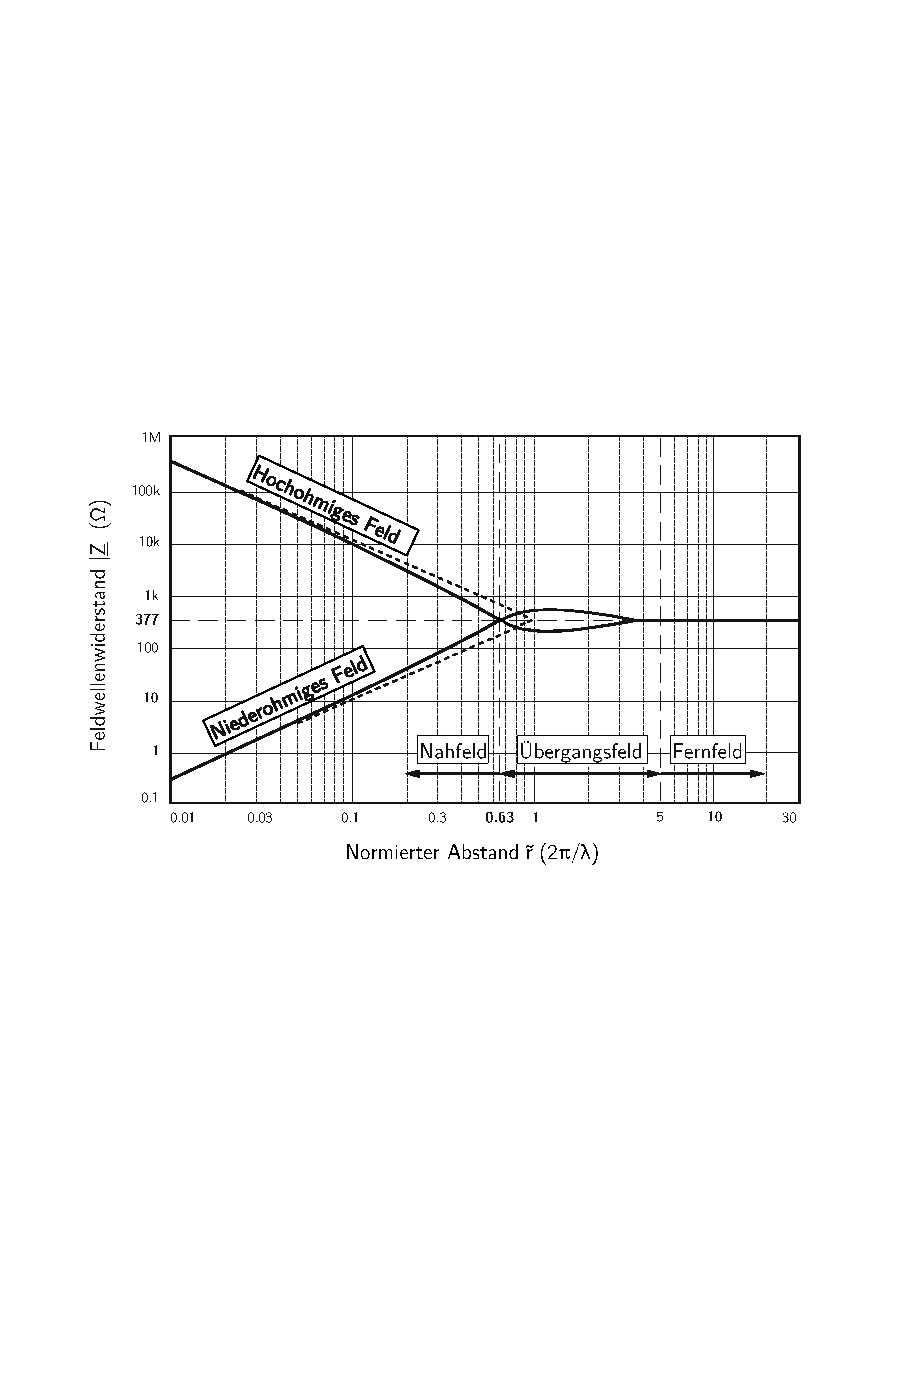
\includegraphics[page=1, width=0.8\textwidth, trim = 2cm 9.5cm 1.5cm 7cm, clip]{Abbildungen/Kapitel2/Feldwellenwiderstand.pdf}};
    \node[below=4cm] at (img) {Normierter Abstand $\tilde r = 2\pi r / \lambda$};
	\node[rotate=90, above=6.5cm] at (img) {Feldwellenwiderstand $|\underline{Z}|$ ($\Omega$)};
    \end{tikzpicture}
    \caption[Verläufe des Feldwellenwiderstandes hoch- und niederohmiger Felder von Stab- und Rahmenantennen in Abhängigkeit des normierten Abstandes von der Feldquelle]{Verläufe des Feldwellenwiderstandes hoch- und niederohmiger Felder von Stab- und Rahmenantennen in Abhängigkeit des normierten Abstandes von der Feldquelle nach~\cite{EMV}}
    \label{fig:2_Feldwellenwiderstand}
\end{figure}


Abhängig von der Art des vorliegenden Feldes unterscheiden sich die Maßnahmen zur Dämpfung und Schirmung maßgeblich voneinander, worauf in den folgenden Abschnitten näher eingegangen wird. Weiterhin ist die Natur des Feldes in der Nähe einer Antenne ebenfalls für Messungen relevant. Für niederfrequente Wechselfelder muss zwischen der Messung elektrischer Felder mit Stabantennen und magnetischer Felder mit Rahmenantennen unterschieden werden. Ab etwa \SI{30}{\mega\hertz} ist die Natur des zu vermessenden Feldes unerheblich für die Bauart der Messantenne, da sich bereits nach kurzem Abstand von der Quelle ein ebenes Wellenfeld ausbildet~\cite{Design_of_shielded_enclosures}.



\subsection{Dämpfung und Absorption}\label{cha:2_sub_Daempfung_und_Absorption}


In verlustbehafteten Medien tritt generell eine Dämpfung der elektrischen und magnetischen Feldstärke einer sich ausbreitenden Welle auf. Absorption bezeichnet dabei eine sehr starke Dämpfung, wobei die Energie der Welle fast vollständig in Wärme umgesetzt wird. Bei einer frequenzabhängigen Dämpfung wird außerdem die Form der Welle verändert. 
\par
\vspace{\linespace}
Die Herleitung der Wellengleichung in Medien endlicher Leitfähigkeit $\sigma > 0$ erfolgt im~\Anhang \ref{Anhang:Herleitung_Wellengleichung}. Dafür kann als Abkürzung der Darstellung die komplexe Wellenzahl $k$

\begin{equation}
    k = \sqrt{\varepsilon \mu \omega^2 - j \omega \sigma \mu}
\end{equation}

eingeführt werden. Je größer der Imaginärteil von k, desto größer wird auch die Phasenverschiebung zwischen den elektrischen und magnetischen Feldgrößen~\cite{EM_Schirmung}. Daher bietet sich eine Zerlegung in Real- und Imaginärteil an

\begin{equation}
    k = \beta - j \alpha \quad \Leftrightarrow \quad jk = \alpha + j\beta \; ,
\end{equation}

wodurch man die Dämpfungskonstante $\alpha$ und die Phasenkonstante $\beta$ erhält. Diese können wiederum aus $k$ zu

\begin{align}
    \alpha &= \omega \sqrt{\frac{\varepsilon \mu}{2}} \sqrt{\sqrt{1+\left(\frac{\sigma}{\omega\varepsilon}\right)^2}-1} \\
    \beta &= \omega \sqrt{\frac{\varepsilon \mu}{2}} \sqrt{\sqrt{1+\left(\frac{\sigma}{\omega\varepsilon}\right)^2}+1}
\end{align}

bestimmt werden~\cite{EM_Schirmung}. Mit diesen Koeffizienten kann eine Interpretation der gewünschten Materialeigenschaften für Dämpfungselemente erfolgen. 
\par
\vspace{\linespace}
Für eine möglichst hohe Dämpfung muss $\alpha$ maximal werden. Dies kann durch eine hohe Leitfähigkeit $\sigma$ und hohe Permeabilität $\mu$ erreicht werden. Die Herausforderung ergibt sich jedoch dadurch, dass sich bei großer Änderung der Leitfähigkeit an einer Grenzfläche die Ausbreitungsbedingungen ggf. so stark ändern, dass die Welle nicht gedämpft, sondern reflektiert wird. Für Absorberelemente ist dies nicht gewünscht, sodass dort eine Dämpfung vor allem durch die Permeabilität erfolgt. Je nach Bauart und Einsatzfrequenz wird dabei dem Magnetfeld Energie durch Ummagnetisierung des Absorbers entzogen, wie es bei Ferritelementen der Fall ist, oder es wird aufgrund der Bauform und mäßiger Leitfähigkeit ein geringer Impedanzsprung hervorgerufen. Letzteres wird mit sogenannten Pyramidenabsorbern erreicht, die häufig aus graphitgetränktem \ac{PU} bestehen und damit ebenfalls hochpermeabel sind~\cite{EM_Schirmung}.
\par
\vspace{\linespace}
Die Höhe der Pyramidenelemente und damit der Winkel der Seitenflächen ist entscheidend für die Absorptionswirkung bei möglichst geringer Reflektion. Je nach Einsatzzweck gibt es auch unterschiedliche Kombinationen von Ferrit- und Pyramidenabsorbern, sowie andere Bauformen für spezielle Anwendungen~\cite{EMV-Support_Produktseite, Telemeter_Produktseite}. Bei Anordnung mehrerer Absorber in Reihe entlang der Ausbreitungsrichtung der zu dämpfenden Welle muss wiederum darauf geachtet werden, dass die Leitfähigkeiten an den Kontaktflächen möglichst genau übereinstimmen. Andernfalls würde man einen Impedanzsprung hervorrufen, der daraufhin ungewollte Reflektionen bewirkt (vgl.~\Abschnitt\ref{cha:2_sub_Verhalten_an_Grenzflächen}). Diese Anpassung kann bei Pyramidenabsorbern bspw. durch den Anteil des Kohlenstoffs im Material geschehen~\cite{EM_Schirmung}.




\subsection{Reflektion}\label{cha:2_sub_Reflektion}


Auf die Ausbreitung von Wellen im Raum müssen natürlich die im \Abschnitt\ref{cha:2_sub_Verhalten_an_Grenzflächen} vorgestellten Grenzflächen von Materialien einen erheblichen Einfluss haben. Da hier die Bedingungen für die Feldvektoren (vgl. \Gleichungen\eqref{eq:2_Flussdichtennormale}) eingehalten werden müssen, muss zu einer durchgelassenen Teilwelle \mbox{(Index \glqq$d$\grqq)} stets eine reflektierte Teilwelle (Index \glqq$r$\grqq) hinzukommen, welche Bestandteil der Wellengleichung ist~\cite{EM_Schirmung}.
\par
\vspace{\linespace}
Für den Grenzfall einer idealleitenden Fläche, auf die eine ebene Welle trifft, muss zum Beispiel die Tangentialkomponente der elektrischen Feldstärke verschwinden~\cite{EM_Schirmung}, was nach \Gleichung \eqref{subeq:2_Feldstaerketangentiale1} zu dem Schluss führt, dass auch die Tangentiale der einfallenden Welle verschwinden muss. Dies kann nur geschehen, indem sich beide gegenseitig auslöschen, was wiederrum nur bei vollständiger Reflektion geschehen kann.
\par
\vspace{\linespace}
Für eine detailliertere Betrachtung lassen sich zwei Fälle unterscheiden. Im Fall \uproman{1} ist das elektrische Feld parallel zur Einfallsebene, während es im Fall \uproman{2} senkrecht dazu steht (vgl.~\Abb \ref{fig:2_Wellenreflektion}). In der Darstellung ist die Zeichenebene die Einfallsebene. Da für die Betrachtung von TEM-Wellen und die Reflektion an metallischen Oberflächen der Fall \uproman{2} relevant ist, soll hier nur dieser betrachtet werden~\cite{EM_Schirmung}.
\par
\vspace{\linespace}

\begin{figure}[ht]
    \centering
    \begin{subfigure}[b]{0.45\textwidth}
        %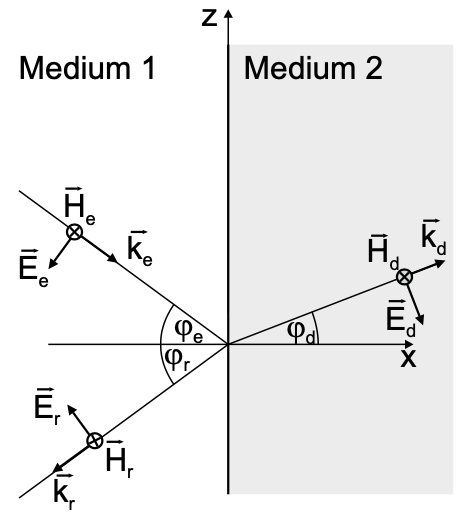
\includegraphics[width=\textwidth]{Abbildungen/Kapitel2/Wellenreflektion_Fall1.png}
        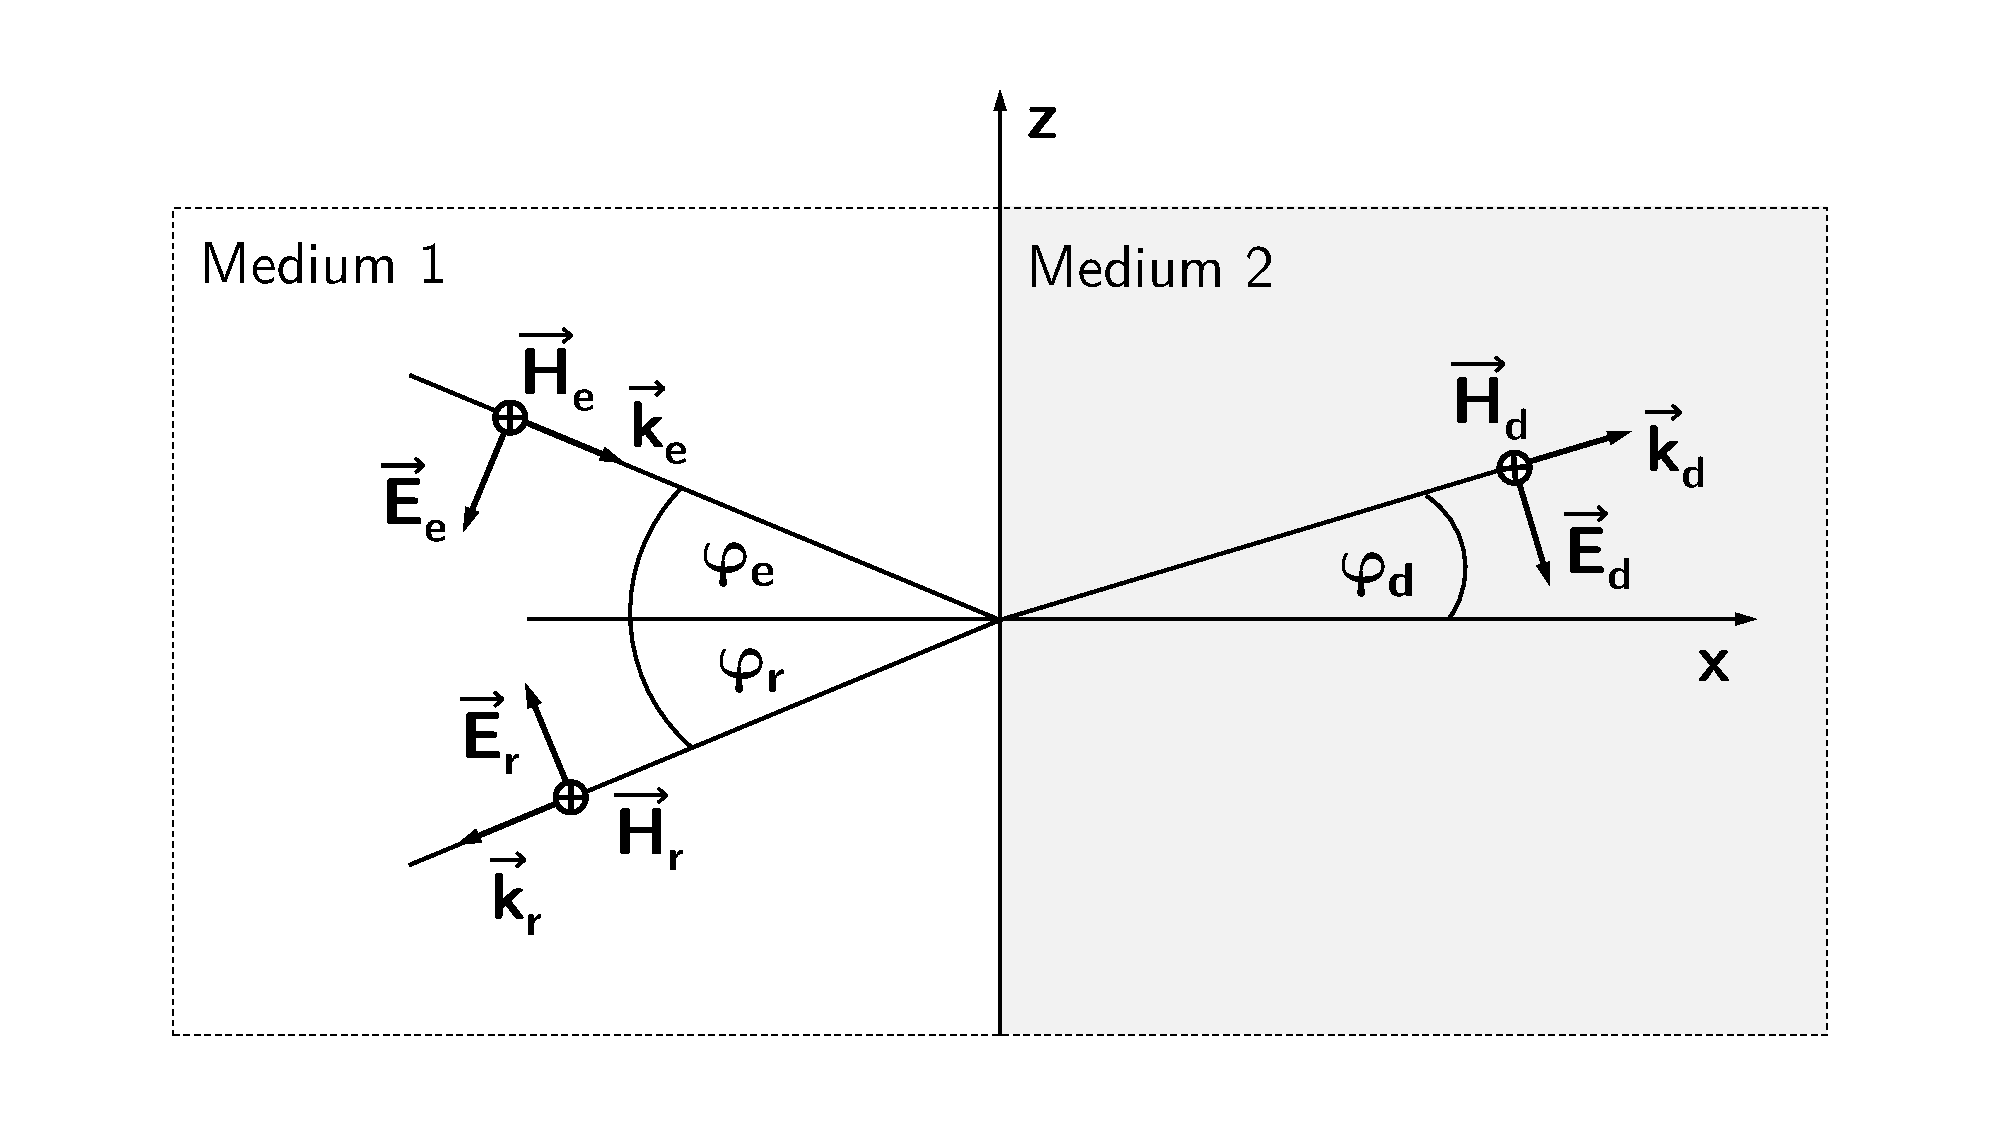
\includegraphics[page = 1, width=\textwidth, trim = 3.5cm 1cm 3.5cm 1cm, clip]{Abbildungen/Kapitel2/Wellenreflektion.pdf}
        \caption{Fall \uproman{1}\label{subfig:2_Wellenreflektion_Fall1}}
    \end{subfigure}
    \hspace{1cm}
    \begin{subfigure}[b]{0.45\textwidth}
        %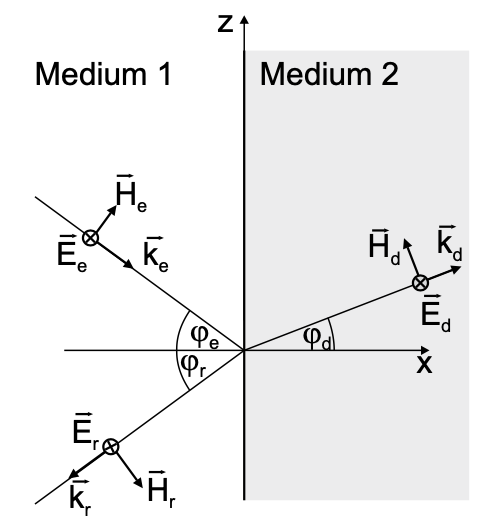
\includegraphics[width=\textwidth]{Abbildungen/Kapitel2/Wellenreflektion_Fall2.png}
        \includegraphics[page = 2, width=\textwidth, trim = 3.5cm 1cm 3.5cm 1cm, clip]{Abbildungen/Kapitel2/Wellenreflektion.pdf}
        \caption{Fall \uproman{2}\label{subfig:2_Wellenreflektion_Fall2}}
    \end{subfigure}
    \caption[Schematische Darstellung des Auftreffens einer elektromagnetischen Welle auf eine Grenzfläche mit reflektierter und durchgelassener Teilwelle]{Schematische Darstellung des Auftreffens einer elektromagnetischen Welle auf eine Grenzfläche mit reflektierter und durchgelassener Teilwelle mit Fallunterscheidung entsprechend der Ausrichtung des elektrischen Feldes zur Einfallsebene nach~\cite{EM_Schirmung}}
    \label{fig:2_Wellenreflektion}
\end{figure}

Für die Feldstärken gelten natürlich die Gleichungen~\eqref{eq:A_Wellengleichungen_mit_Leitfaehigkeit} aus der Herleitung der Wellengleichung im \Anhang \ref{Anhang:Herleitung_Wellengleichung}. Angewandt auf die dargestellten geometrischen Verhältnisse ergibt sich für die einfallende Welle (Index \glqq$e$\grqq)~\cite{EM_Schirmung}:

\begin{align}
    \vec E_e &= E_0 e^{-j\vec k_e \vec r} \vec e_y \\
    \vec H_e &= \frac{E_0}{Z_1} \sin{\varphi_e} e^{-j \vec k_e \vec r} \vec e_x + \frac{E_0}{Z_1} \cos{\varphi_e} e^{-j \vec k_e \vec r} \vec e_z \\
    \vec k_e &= k_1 \cos{\varphi_e} \vec e_x - k_1 \sin{\varphi_e} \vec e_z \\
    Z_1 &= \frac{E_0}{H_0}
\end{align}

als Ausgangspunkt für die Betrachtung der Reflektion an einer Grenzfläche. Dabei ist zu berücksichtigen, dass hier die Ausbreitung, im Gegensatz zu \Gleichungen \eqref{eq:A_Wellengleichungen_mit_Leitfaehigkeit}, nicht in Richtung der x-Achse erfolgt, sondern entlang einer beliebigen Richtung. Dafür kann der Ortsvektor $\vec r$ als Ausgangspunkt und der Wellenzahlvektor $\vec k$ als Richtungsvektor mit
$|\vec k| = k = \sqrt{\varepsilon \mu \omega^2 - j \omega \sigma \mu} $ eingeführt werden~\cite{EM_Schirmung}. \par \vspace{\linespace} Analog kann für die reflektierte und die durchgelassene Teilwelle mit dem Reflektionsfaktor $R_{\uproman{2}}$ und dem Durchlassfaktor $D_{\uproman{2}}$

\begin{align}
    \vec E_r &= E_0 R_{\uproman{2}} e^{-j\vec k_r \vec r} \vec e_y \\
    \vec H_r &= \frac{E_0}{Z_1} R_{\uproman{2}} \sin{\varphi_r} e^{-j \vec k_r \vec r} \vec e_x - \frac{E_0}{Z_1} R_{\uproman{2}} \cos{\varphi_r} e^{-j \vec k_r \vec r} \vec e_z \\
    \vec k_r &= - k_1 \cos{\varphi_r} \vec e_x - k_1 \sin{\varphi_r} \vec e_z \\
    \vec E_d &= E_0 D_{\uproman{2}} e^{-j\vec k_d \vec r} \vec e_y \\
    \vec H_d &= \frac{E_0}{Z_2} D_{\uproman{2}} \sin{\varphi_d} e^{-j \vec k_d \vec r} \vec e_x + \frac{E_0}{Z_2} D_{\uproman{2}} \cos{\varphi_d} e^{-j \vec k_d \vec r} \vec e_z \\
    \vec k_d &= k_2 \cos{\varphi_d} \vec e_x - k_2 \sin{\varphi_d} \vec e_z
\end{align}

geschrieben werden. Unter Zuhilfenahme der Gesetzmäßigkeiten an Grenzflächen~\eqref{eq:2_Feldstaerketangentiale} für die Stelle $x=0$, lassen sich folgende Ausdrücke für den Reflektions- und den Durchlassfaktor finden, die das Verhältnis der beiden Teilwellen nach Auftreffen auf eine Grenzschicht beschreiben:

\begin{align}
    R_{\uproman{2}} &= \frac{Z_2 \cos{\varphi_e} - Z_1 \cos{\varphi_d}}{Z_2 \cos{\varphi_e} + Z_1 \cos{\varphi_d}} \\
    D_{\uproman{2}} &= \frac{2 Z_2 \cos{\varphi_e}}{Z_2 \cos{\varphi_e} + Z_1 \cos{\varphi_d}} \\ 
    1 &= D_{\uproman{2}} - R_{\uproman{2}} = D_{\uproman{2}} \frac{Z_1 \cos{\varphi_d}}{Z_2 \cos{\varphi_e}} + R_{\uproman{2}} \; .
\end{align}

Für den Fall, dass an der Grenzfläche kein Materialübergang stattfindet ($Z_1 = Z_2$), gilt $\varphi_e = \varphi_d$ und damit $R_{\uproman{2}} = 0$ und $D_{\uproman{2}} = 1$, das bedeutet die Welle wird nicht gebeugt und es findet keine Reflektion statt. Handelt es sich bei Medium 2 dagegen um einen idealen Leiter mit $Z_2 = 0 \neq Z_1$, so wird $D_{\uproman{2}} = 0$ und $R_{\uproman{2}} = -1$, was entsprechend der Erwartung heißt, dass eine eintreffende Welle an einer idealisierten metallischen Oberfläche vollständig reflektiert wird~\cite{EM_Schirmung}. 






